\documentclass[12pt,a4paper]{article}
\usepackage[utf8]{inputenc}
\usepackage{graphicx}
\usepackage{float}
\usepackage{subcaption}
\usepackage[margin=1in]{geometry}
\usepackage{hyperref}
\hypersetup{
  pdfborder = {0 0 0}
}
\usepackage[
backend=biber,
style=alphabetic,
]{biblatex}

\addbibresource{PhSp.bib}

\graphicspath{{./PhSp/}}
\DeclareGraphicsExtensions{.pdf,.jpeg,.jpg,.png}

\usepackage{amsmath} % equations
\usepackage{fancyhdr} % nicer page header

\setlength{\parindent}{0pt} % no paragraph indents
\setlength{\parskip}{1em} % paragraphs separated by one line

\newcommand\experiment{N-Body Simulations with REBOUND} %%%%% experiment name
\newcommand\groupno{Group 3}       %%%%% group number
\newcommand\names{Pratyush Singh,\\
                  Proshmit Dasputpa\\}        %%%%% full names
\newcommand\expdate{07/03/2025}    %%%%% date of experiment day

\begin{document}
\begin{titlepage}
   \begin{center}
        \vspace*{3cm}
        \Huge{\experiment}
				
        \vspace{0.5cm}
        \LARGE{Lab course protocol}
				
        \vspace{3 cm}
        \Large{\groupno}
				
        \vspace{0.25cm}
        \large{\names}
				
        \vspace{2 cm}
        \Large{\expdate}
				
        \vspace{0.25 cm}
        \Large{Advanced lab course in astronomy\\
				Eberhard Karls Universit\"at T\"ubingen}
				
				\vspace{0.1 cm}
        \Large{WiSe 2024/25}
				
       \vfill
    \end{center}
\end{titlepage}

\pagestyle{fancy}
\fancyhf{}
\setlength{\headheight}{14.5pt}
\lhead{\groupno; \experiment}

\section*{Abstract}
This is optional, but never longer than half a page.

\tableofcontents
\newpage

\setcounter{page}{1}
\pagestyle{fancy}
\fancyhf{}
\rhead{\thepage}
\lhead{\groupno; \experiment}

\section{Introduction}\label{sec:intro} % labels allow references, particularly important for figures and tables
In the experiment, we will use the 80 cm telescope of the IAAT to study photometry and spectroscopy. These two topics are fundamental to observational astronomy 
and are used to study the properties of stars, galaxies and other bodies. In photometry, we aim to determine the brightness of several stars in the star cluster M37 in 
the B and V filters which will be used to determine the age and distance to the cluster. In spectroscopy, we will look at the spectrum of one (or both) of the stars of 
the Castor binary system and identify the $H\alpha$ spectral line (and more).


\section{Theory}\label{sec:theory}
\subsection{Telescope}
  Telescopes are used in observing the EM radiation emitted by distant sources. Telescopes collect light from a certain direction and are used to apply an angular magnification to the image. The two major types of telescopes are 
  the lens telescope (the refractor) or the mirror telescope (the reflector). The amount of light that a telescope can gather depends on the `aperture' of the telescope $D$. The ratio of this and the focal length
  $F$ is the aperture ratio $F/D$. A telescope with a higher aperture ratio will produce a brighter image. The magnification of the telescope is determined by the ratio of the main mirror focal length $F$ and the eye piece focal length
  $f$. i.e. $M = F/f$. 
  \\
  The resolving power of a telescope is its ability to distinguish between two nearby sources and is defined by the Rayleigh criterion:
  \begin{equation}
    \alpha = 1.22 \frac{\lambda}{D}
  \end{equation}

  Unfortunately due to atmospheric effects, the resolving power is slightly worse and is limited to $\alpha = \lambda/D$. For a telescope with an aperture of 80 cm, the resolving power
  at $\lambda = 5700 \AA$  is \dots.
  \subsubsection{The 80 cm Telescope}
    The 80 cm telescope is located in Sand, Tübingen and was built in 2003. It is a mirror telescope in Cassegrain configuration with Nasmyth focus. It has an aperture of 80 cm and 
    a focal length of 6.4 m. For slewing, the telescope is mounted on an equatorial open fork mount and can move to focus on any point in the sky in its line of sight.
    \begin{figure}[H]
      \centering
      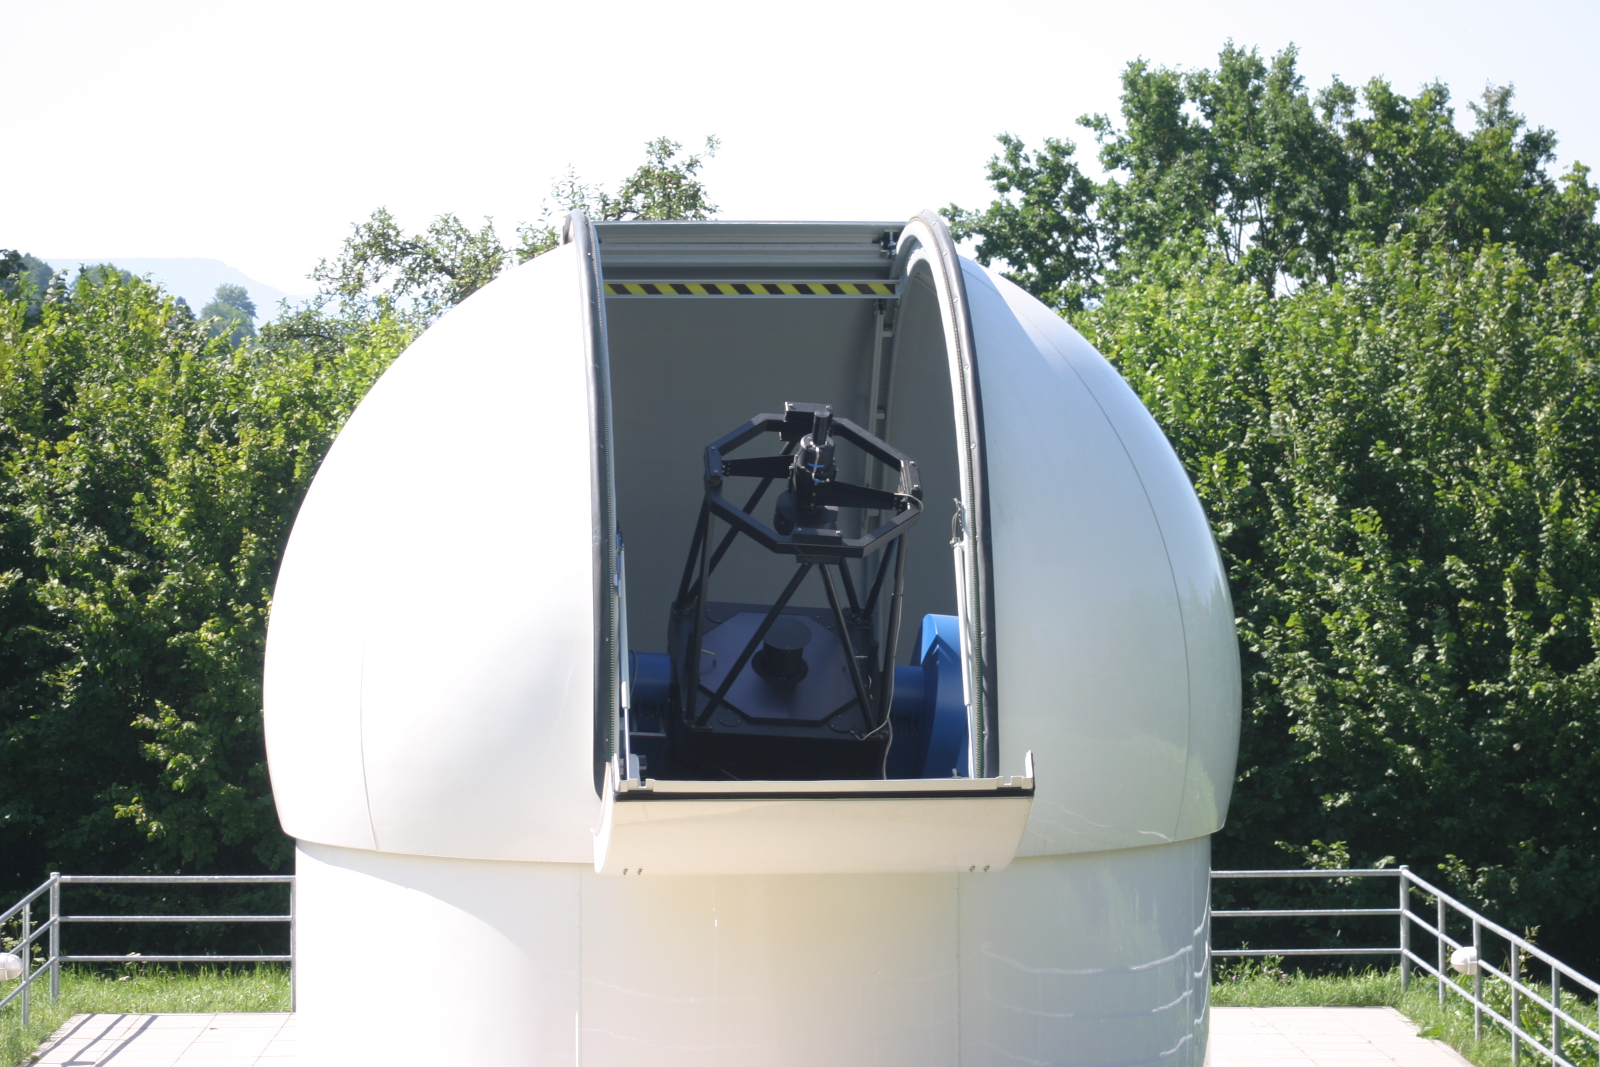
\includegraphics[width=0.5\textwidth]{./Pictures/2004_img_0962.jpg}
      \caption{The 80 cm telescope at the IAAT.}
      \label{fig:80cm}
    \end{figure}
    In figure \ref{fig:80cm_lp} we can see the path light has to travel to reach the focus points. The starlight enters from above and is reflected by the primary mirror towards the 
    secondary mirror. It reflects back the light towards a plain mirror which focuses the light on either the left or the right focus. This configuration (Cassegrain-Nasmyth) allows a smaller size of the telescope
    (around 3 m) for a larger focal length of 6.4 m. The Nasmyth focus also is beneficial for mounting heavy instruments that don't need to be moved with the declination axis. 
    \begin{figure}[H]
      \centering
      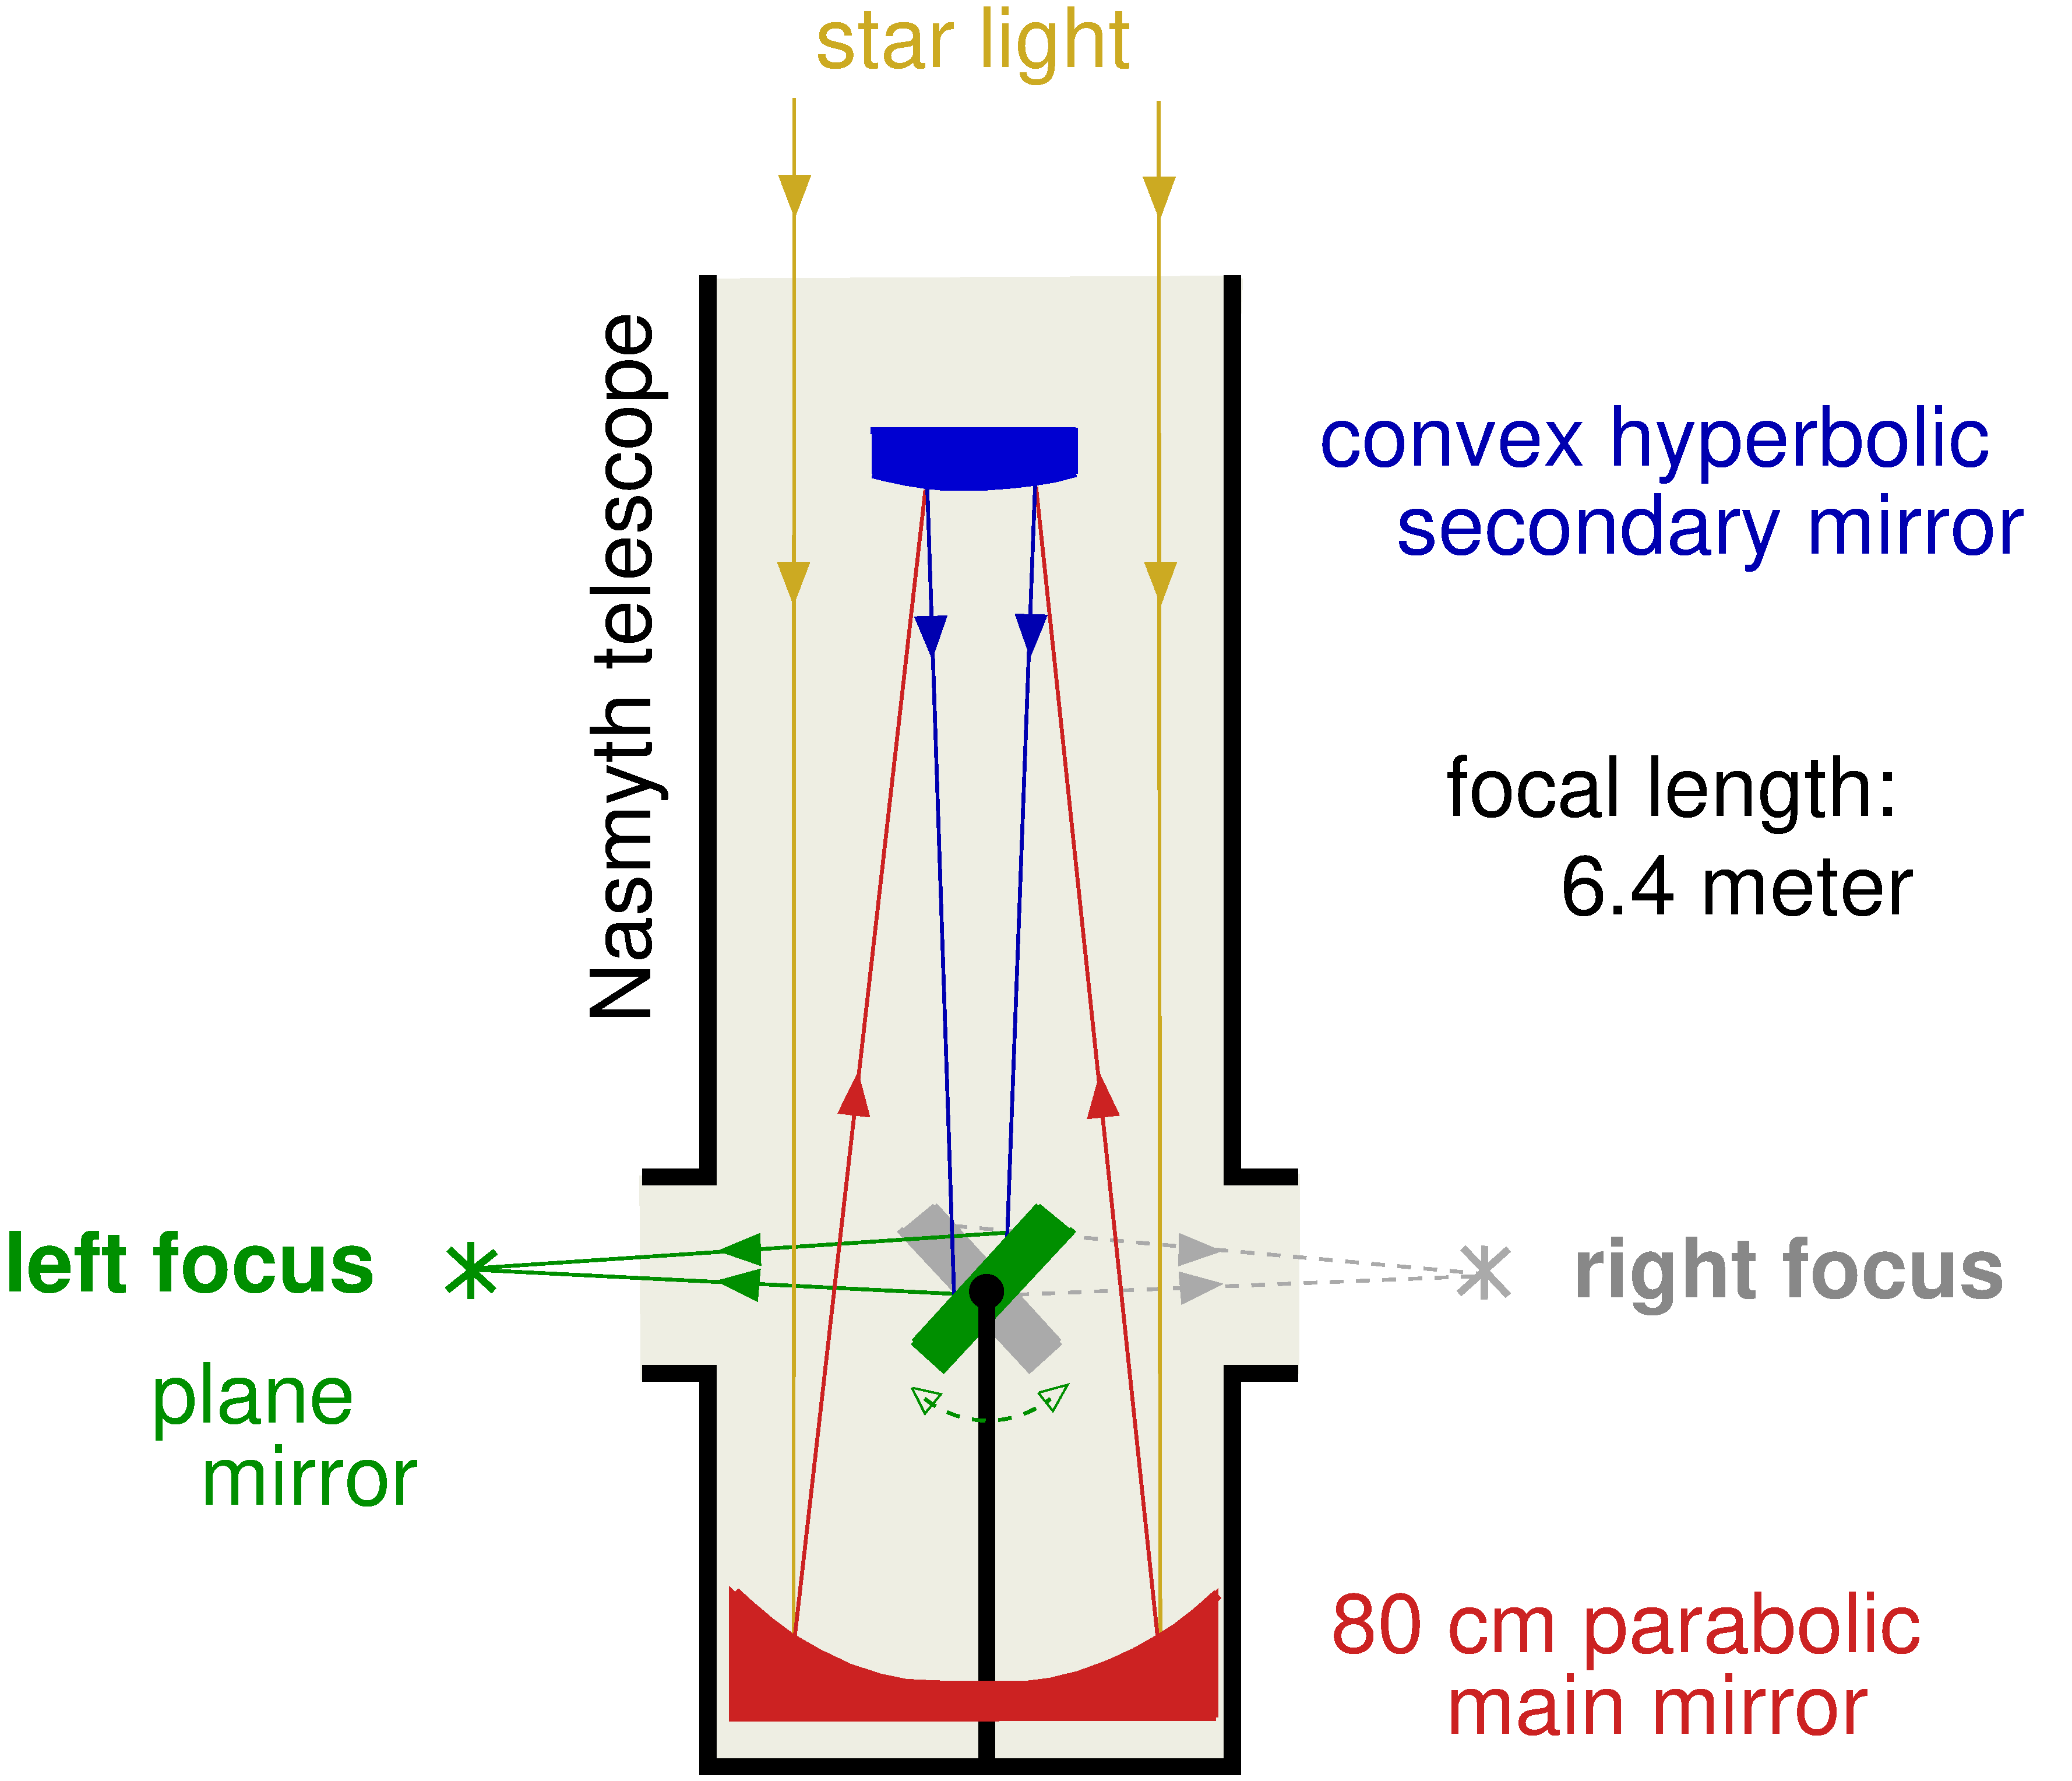
\includegraphics[width=0.5\textwidth]{Pictures/Nasmyth2.pdf}
      \caption{The light path of the 80 cm telescope.}
      \label{fig:80cm_lp}
    \end{figure}

  \subsection{CCD}
  \subsection{Photometry}
  \subsection{Spectroscopy}
\section{Experiment}

\section{Conclusions}
An important section in which you should critically review the experiment and its results. Mention also parts that did not work out as expected, but keep a neutral to positive view. This can span from a few sentences to half a page.

\setcounter{secnumdepth}{0}

\printbibliography
\appendix
\section{Appendix}
\subsection{Code}
\label{code}
Please attach here your original handwritten notes and other documents created during the experiment.

\end{document}

